\section{Previous work}

\begin{frame}
    \frametitle{Where were we?}

    \centering
    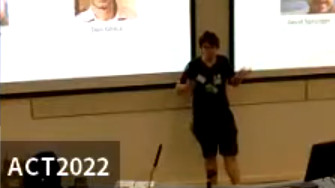
\includegraphics[width=0.75\textwidth]{imgs/act2022}

\end{frame}

\begin{frame}
    \frametitle{What is the meaning?}

    \centering
    \Large

    What are the \alert{denotational semantics} of digital circuits?

    \await

    Certain kinds of \alert{stream functions}!
    \[
        f(v_0 \streamcons v_1 \streamcons v_2 \streamcons \dots)
        =
        w_0 \streamcons w_1 \streamcons w_2 \streamcons \dots
    \]

    \await

    \LARGE

    \alert{Denotational} equivalence
    \[\left\llbracket\iltikzfig{strings/category/f}[colour=seq]\right\rrbracket
        =
        \left\llbracket\iltikzfig{strings/category/f}[box=g,colour=seq]\right\rrbracket
        \Rightarrow
        \iltikzfig{strings/category/f}[colour=seq]
        \approx
        \iltikzfig{strings/category/f}[box=g,colour=seq]
    \]
\end{frame}
\begin{frame}
    \frametitle{Guards, guards!}

    \centering
    \Large

    We can also \alert{eliminate non-delay-guarded feedback}
    \normalsize
    \[
        \dsptikzfig{strings/traced/trace-rhs}[colour=comb]
        \approx
        \dsptikzfig{circuits/instant-feedback/general}
    \]

    (Kleene fixpoint theorem)

\end{frame}
\begin{frame}
    \frametitle{We want something different}

    \centering
    \Large

    Denotational equivalence obscures the \alert{structure} of terms

    \await

    We want to reason more \alert{syntactically}

    \vspace{1em}

    \LARGE
    \pause
    \begin{minipage}{0.45\textwidth}
        \centering
        Operational
        semantics

        \vspace{0.5em}

        \large
        a bit has changed
    \end{minipage}
    \pause
    \begin{minipage}{0.45\textwidth}
        \centering
        Algebraic
        semantics

        \vspace{0.5em}

        \large
        (pretty much) new
    \end{minipage}
\end{frame}